%%
%% i6-style slides
%% customized for kim
%%

\documentclass[11pt, a4paper, landscape]{article}
\usepackage[userlastpage,triangle,utf-8,noblackslide]{NeyDreuwSlides_Oct08}
\usepackage{snapshot}
\usepackage{mathtools}
\usepackage{amssymb,amsmath,amsthm,enumitem}
\usepackage[caption]{subfig}
%\usepackage{algorithm}
%\usepackage[noend]{algpseudocode}
\usepackage[ruled,linesnumbered]{algorithm2e}
\usepackage{bm}
	\usepackage[
	singlelinecheck=false % <-- important
	]{caption}

% slides tunning
% \setlength{\footskip}{0pt} % default ist +30pt - negative Werte nicht moeglich
% \setlength{\headsep}{-10pt} % default ist +25pt - negative Werte moeglich
% \addtolength{\topmargin}{-5mm} % bewegt den gesamten Inhalt der Seite nach oben
% \setlength{\textheight}{170mm} % wenn moeglich nicht veraendern, beinflusst den Inhalt der Seiten und somit auch die Anzahl der Seiten!

% math operators and
% symbols %%%%%%%%%%%%%%%%%%%%%%%%%%%%%%%%%%%%%%%%%%%%%%%%%%%
\newcommand*{\nat}{\ensuremath{\rm I\!N}\xspace}
\newcommand*{\rel}{\ensuremath{\rm I\!R}\xspace}
\newcommand*{\argmin}{\ensuremath{\operatornamewithlimits{argmin}}\xspace}
\newcommand*{\argmax}{\ensuremath{\operatornamewithlimits{argmax}}\xspace}
\newcommand*{\congmod}{\ensuremath{\operatornamewithlimits{\cong}}\xspace}
\newcommand*{\invers}{\ensuremath{\frac{1}}\xspace}
\newcommand*{\ra}{\ensuremath{\Rightarrow}\xspace}

%%%%%%%%%%%%%%%%%%%%%%%%%%%%%%%%%%%%%%%%%%%%%%%%%%%%%%%%%%%%%%%%%%%%%%%%%%%%%%%%
% custom packages
\usepackage{fancyvrb} %%% fancy verbatim to enable coloring within verbatim environments
\usepackage{bbding}
\usepackage{multirow}
\usepackage{graphicx}
\usepackage{tikz}

\newcolumntype{C}[1]{>{\centering\arraybackslash}p{#1}}
\newcolumntype{L}[1]{>{\raggedright\arraybackslash}p{#1}}

\renewcommand{\arraystretch}{1.5}

%%%%%%%%%%%%%%%%%%%%%%%%%%%%%%%%%%%%%%%%%%%%%%%%%%%%%%%%%%%%%%%%%%%%%%%%%%%%%%%%
% main title of the work (used for \TitlePage)
\renewcommand*{\title}{Unsupervised Learning of Neural Lexicon and Cross-lingual Word Embedding}
% short title (used for \lfoot)
\renewcommand*{\titleshort}{Unsupervised Learning of Cross-lingual Word Embedding}
% (used for \TitlePage)
\renewcommand*{\occasion}{Master Thesis Mid-term Talk\\}
% short occasion title (used for \rfoot)
\renewcommand*{\occasionshort}{}
% default is \today (used for \TitlePage and \rfoot)
\renewcommand*{\date}{\today}
% all the authors of the work, can be long (used for \TitlePage)

\renewcommand*{\author}{Jiahui Geng}

% all the authors of the work, should be short (used for \lfoot)
\renewcommand*{\authorshort}{J. Geng:\xspace}
% all email address(es) of the authors (used for \TitlePage)
\renewcommand*{\email}{\url{jiahui.geng@rwth-aachen.de}}
% the author(s) who presented the work (used for \TitlePage)
\renewcommand*{\mainauthor}{Jiahui Geng}
% presenter mail address(es) (used for \FinalPage)
\renewcommand*{\mainauthoremail}{\url{jgeng@cs.rwth-aachen.de}}
% web address (used for \TitlePage _and_ \FinalPage)
\renewcommand*{\www}{http://www.hltpr.rwth-aachen.de/}
% keywords, can be used for PDF summary
\newcommand*{\keywords}{}

% will be set into the PDF document summary
\hypersetup{ pdftitle={\title}, pdfsubject={\occasion},
	pdfauthor={\author}, pdfkeywords={\keywords}, pdfpageduration = 2,
	pdfpagetransition = {Box /M /O /D 1}, }


%%%%%%%%%%%%%%%%%%%%%%%%%%%%%%%%%%%%%%%%%%%%%%%%%%%%%%%%%%%%%%%%%%%%%%%%%%%%%%%%
\listfiles
%%%%%%%%%%%%%%%%%%%%%%%%%%%%%%%%%%%%%%%%%%%%%%%%%%%%%%%%%%%%%%%%%%%%%%%%%%%%%%%%
\begin{document}
	%\setlength{\abovedisplayskip}{5pt}
	%\setlength{\belowdisplayskip}{3pt}
	%%%%%%%%%%%%%%%%%%%%%%%%%%%%%%%%%%%%%%%%%%%%%%%%%%%%%%%%%%%%%%%%%%%%%%%%%%%%%%%%
	\TitlePage
	
	%%%%%%%%%%%%%%%%%%%%%%%%%%%%%%%%%%%%%%%%%%%%%%%%%%%%%%%%%%%%%%%%%%%%%%%%%%%%%%%%%%%%%%% 
	\NewPage
	
	\headline {Outline}
	
	\vfill
	\begin{description}
		\item Introduction
		\item Literature
		\item Cross-lingual word embedding
		\begin{itemize}
			\item Supervised learning
			\item Unsupervised learning
		\end{itemize}
		\item Sentence Translation with cross-lingual word embedding
		\begin{itemize}
			\item Context-aware beam search
			\item Denoising autoencoder
		\end{itemize}
		\item Experiments

		\item Outlook
	\end{description}
	\vfill
	
	%%%%%%%%%%%%%%%%%%%%%%%%%%%%%%%%%%%%%%%%%%%%%%%%%%%%%%%%%%%%%%%%%%%%%%%%%%%%%%%%%%%%%%%
	\NewPage
	\headline {Introduction}
	
	\vfill
	\begin{description}
		\item Motivation
		\begin{itemize}
			\item Building a machine translation system requires lots of bilingual data
			\item Cross-lingual word embedding offers elegant word matches between languages
			\item Unsupervised MT relies on back-translation which needs a long training time
		\end{itemize}
		\item Goals
		\begin{itemize}
			\item Study training details of cross-lingual word embedding
			\item Build a good unsupervised MT efficiently: combine with other models
			\item Improve the unsupervised learning algorithm for cross lingual word embedding
		\end{itemize}
		
	\end{description}
	\vfill
	

	
	
	
	%%%%%%%%%%%%%%%%%%%%%%%%%%%%%%%%%%%%%%%%%%%%%%%%%%%%%%%%%%%%%%%%%%%%%%%%%%%%%%%%%%%%%%%
	\NewPage
	\headline {Literature}
	
	\vfill
	Unsupervised cross-lingual embedding
	\begin{itemize}
		\item 	\cite{conneau2017word} Word translation without parallel data
		\begin{itemize}
		\item Implementation of GANs: discriminator trained to distinguish between two distributions while generator fools discriminator 
		\end{itemize}	
		\item 	\cite{artetxe2017learning} Learning bilingual word embeddings with (almost) no bilingual data
		\begin{itemize}
			\item A self-learning framework combining embedding mapping and dictionary induction techniques, needs seed dictionary to start
		\end{itemize}	    
		\item \cite{hoshen2018iterative} An Iterative Closest Point Method for Unsupervised Word Translation	    
		\begin{itemize}
			\item Iterative closest point method for embedding mapping learning
		\end{itemize}	    
	\end{itemize}
	
	
	
	
	
	
	\vfill
	
	%%%%%%%%%%%%%%%%%%%%%%%%%%%%%%%%%%%%%%%%%%%%%%%%%%%%%%%%%%%%%%%%%%%%%%%%%%%%%%%%%%%%%%%
	\NewPage
	\headline {Literature}
	
	\vfill
	Unsupervised machine translation
	\begin{itemize}
		\item 	\cite{artetxe2017unsupervised} Unsupervised Neural Machine Translation
		\item \cite{lample2017unsupervised} Unsupervised Machine Translation Using Monolingual Corpora Only
		\begin{itemize} 
			\item Seq2seq model with shared encoder and decoder for both languages, also with denoising autoencoder and back-translation
		\end{itemize}
		
		\item \cite{artetxe2017unsupervised} Phrase-Based \& Neural Unsupervised Machine Translation
		\begin{itemize}
			\item Simplifies the architecture and loss function for unsupervised NMT and propose a phrase-based SMT with back-translation
		\end{itemize}	
		

	\end{itemize}
	
	\vfill



	%%%%%%%%%%%%%%%%%%%%%%%%%%%%%%%%%%%%%%%%%%%%%%%%%%%%%%%%%%%%%%%%%%%%%%%%%%%%%%%%%%%%%%%
	\NewPage
	\headline{Cross-lingual Word Embedding}
	\vfill
	
	Definition
	\begin{itemize}
		\item Word embedding of multiple languages in a joint embedding space		
		\item Linear mapping from source embedding to target embedding (this work)
	\end{itemize}
	\begin{figure}
	\begin{minipage}[b]{0.55\textwidth}
	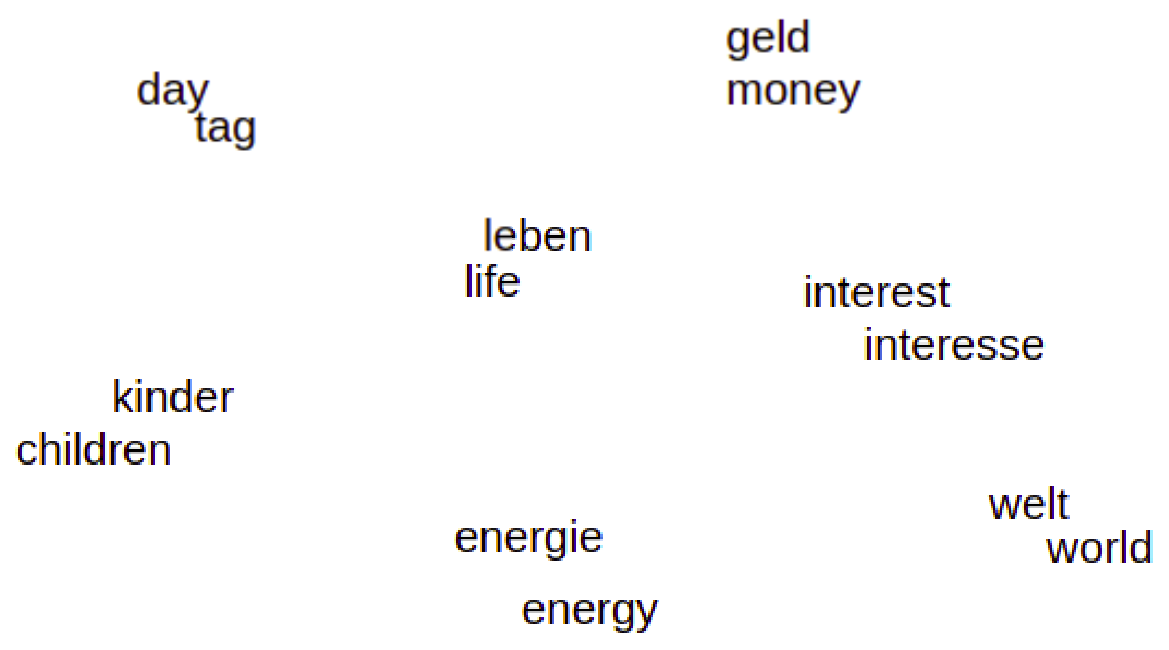
\includegraphics[width=14cm]{crossembedding}
	\caption{cross-lingual word embedding}	
	
	\end{minipage}
	\begin{minipage}[b]{0.4\textwidth}
		\centering
		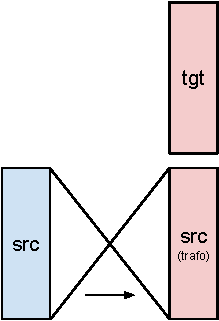
\includegraphics[width=0.5\textwidth]{cross-embed}
		\caption{cross-lingual mapping}

	\end{minipage}	
	\end{figure}

	\vfill
	%%%%%%%%%%%%%%%%%%%%%%%%%%%%%%%%%%%%%%%%%%%%%%%%%%%%%%%%%%%%%%%%%%%%%%%%%%%%%%%%%%%%%%
	\NewPage
	\headline{Cross-lingual Word Embedding}
	\vfill
	Roles in unsupervised neural machine translation 
	\begin{itemize}
		\item Shared latent representations
		\begin{itemize}
			\item Shared encoder for producing a language independent representation
		\end{itemize}	
		\item As word or phrase table for translation\\
	\end{itemize}	
	This work
	\begin{itemize}
	\item Formulate a straightforward way to combine
		a language model with cross-lingual
		word similarities \\
	\end{itemize}
		
	Training Methods
	
	\begin{itemize}
		\item Mapping-based approaches (this work)

		\item Pseudo-multi-lingual corpora-based approaches

		\item Joint methods

	\end{itemize}

	\vfill


	
	
	%%%%%%%%%%%%%%%%%%%%%%%%%%%%%%%%%%%%%%%%%%%%%%%%%%%%%%%%%%%%%%%%%%%%%%%%%%%%%%%%%%%%%%
	\NewPage
	\headline{Cross-lingual Word Embedding}
	\vfill
	Mapping based approaches
	\begin{itemize}
	\item Learn monolingual embedding separately
	\begin{itemize}
		\item Skip-gram model 
	\end{itemize}
	\item Learn linear mapping between embedding spaces	
	\begin{itemize}
		\item Supervised learning
		\begin{itemize}
			\item Procrustes analysis
		\end{itemize}
		\item Unsupervised learning
		\begin{itemize}
			\item Iterative self-learning framework 			
			\item Adversarial learning
		\end{itemize}
	\end{itemize}
	\item Synthetic dictionary induction
	\begin{itemize}
		\item Nearest neighbor search
	\end{itemize}
	
\end{itemize}
	\vfill
	
	
	
	%%%%%%%%%%%%%%%%%%%%%%%%%%%%%%%%%%%%%%%%%%%%%%%%%%%%%%%%%%%%%%%%%%%%%%%%%%%%%%%%%%%%%%%
	\NewPage
	\headline{Monolingual Embedding}
	\vfill



	\texttt{Fasttext} \cite{bojanowski2017enriching}
	\begin{itemize}
		\item Essentially an extension of skip-gram/CBOW model
		\item Treat each word as compound of character ${n}$-grams
		\item Learn the internal structure of words\\
		
		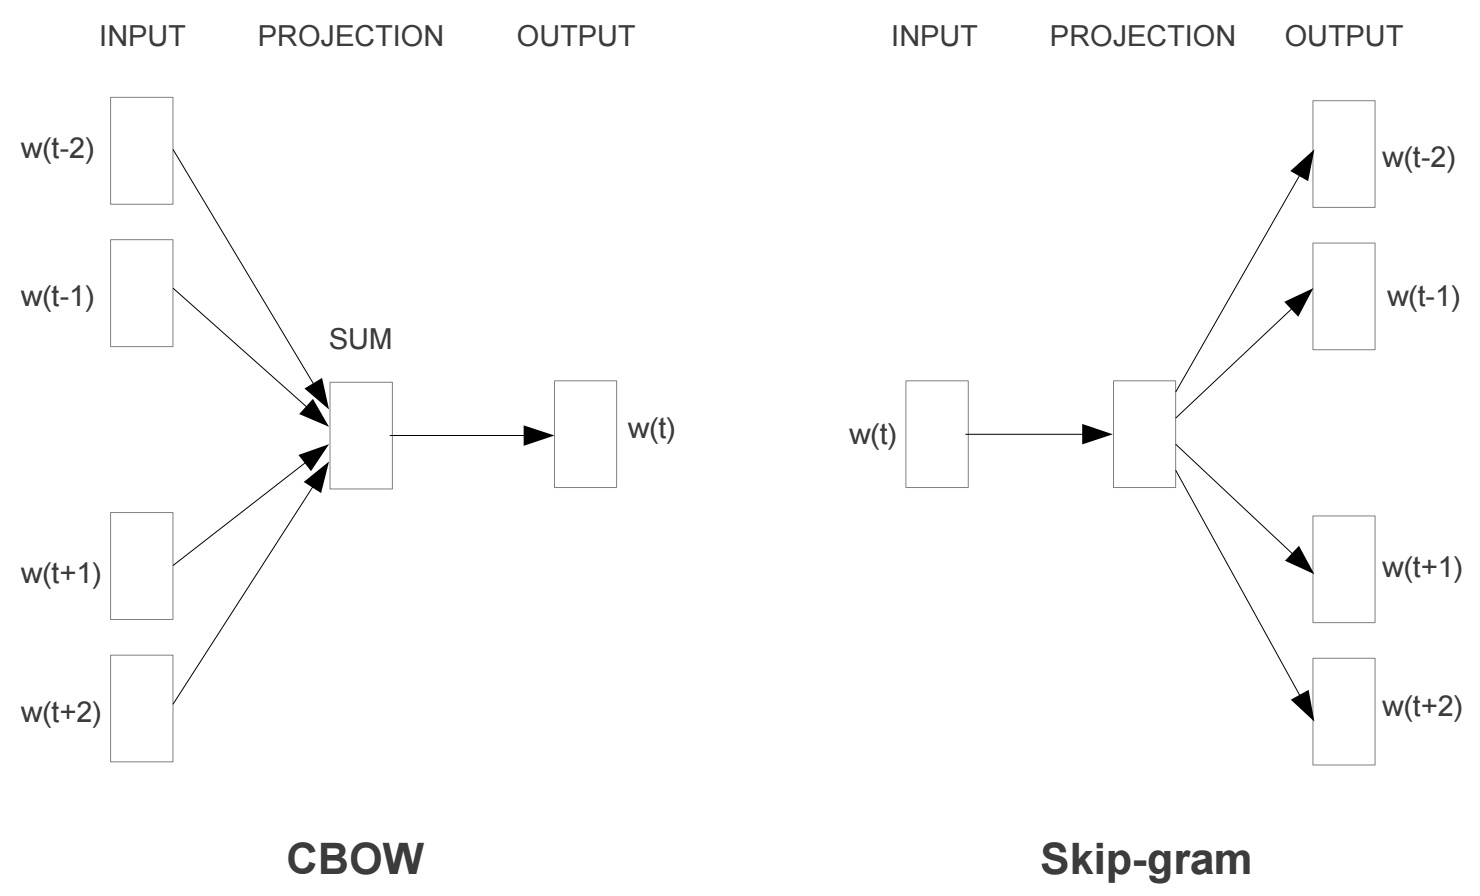
\includegraphics[width=0.7\linewidth]{skip}
		\centering
	\end{itemize}
	
	
	\vfill	
	%%%%%%%%%%%%%%%%%%%%%%%%%%%%%%%%%%%%%%%%%%%%%%%%%%%%%%%%%%%%%%%%%%%%%%%%%%%%%%%%%%%%%%%
	\NewPage
	\headline{Learning with Parallel Dictionary}
	\vfill
	Assume given
	\begin{itemize}
		\item Word embedding \\
		trained  independently for each language on monolingual corpora
		\item Bilingual dictionary \\
		a known dictionary with pairs of words ${ \{ \bm{f}, \bm{e} \} }$ size $N$ 
	\end{itemize}
	
	
	
	Learn a linear mapping ${W \in \mathbb{R}^{d \times d}}$ such that
	\[W^*= \argmin\limits_{W \in \mathbb{R}^{d \times d}} {\sum_{n=1}^{N} {\lVert Wf_n -e_n \rVert}^2} \]
	\begin{itemize}
		\item ${d:}$ Dimension of embedding
		\item $f_n, e_n \in \mathbb{R}^d $: the embedding pair of corresponding word pair in the dictionary
	\end{itemize}
	\vfill
	
	
	
	%%%%%%%%%%%%%%%%%%%%%%%%%%%%%%%%%%%%%%%%%%%%%%%%%%%%%%%%%%%%%%%%%%%%%%%%%%%%%%%%%%%%%%%
	\NewPage
	\headline{Procrustes Analysis}
	\vfill
	Constrain ${W}$ to be an orthogonal matrix
	\begin{itemize}
		\item Enforce monolingual invariance
		
		\item Simplify the problem as the Procrustes problem
		
		\begin{itemize}
			\item A closed-form solution obtained from SVD
			\item $E$, $F \in \mathbb{R}^{d\times N}$ denote embedding projection of word pairs ${\{e,f\}}$
		\end{itemize}
		
		\[ W^* = \argmin\limits_{W \in \mathbb{R}^{d \times d}} {\lVert WF-E\lVert}_F^2  =  UV^T\]
		\[ U\varSigma V^T =  \textrm{SVD}(EF^T)\]
		
		\item Can be efficiently computed in linear time  w.r.t. seed dictionary size $N$
	\end{itemize}
	\vfill
	
	%%%%%%%%%%%%%%%%%%%%%%%%%%%%%%%%%%%%%%%%%%%%%	
	\NewPage
	\headline{Learning without Parallel Dictionary}
	\vfill
	Problem
	\begin{itemize}
		\item Large dictionary not readily available for many language pairs\\
	\end{itemize}
	Self-learning framework \cite{artetxe2017learning}
	\begin{enumerate}
		\item Given source and target embedding ${\mathcal{F}}$ ${\mathcal{E}}$ , seed dictionary $D$
		\item Learn mapping with dictionary $D$
		\item Induce dictionary $D^{\prime}$ according to mapping
		\item ${D:=D^{\prime}}$ and repeat step $2$, $3$ until converges\\
	\end{enumerate}
	
	Performance
	\begin{itemize}
		\item Works with initial dictionary		
		\item Achieves comparable accuracy as supervised method
		\item Stuck in a poor local optimum without initial dictionary
	\end{itemize}
	
	\vfill
	
	%%%%%%%%%%%%%%%%%%%%%%%%%%%%%%%%%%%%%%%%%%%%%%%%%%%%%%%%%%%%%%%%%%%%%%%%%%%%%%%%%%%%%%%
	\NewPage
	\headline{Learning without Parallel Dictionary}	
	\vfill

		
	
	Methods
	\begin{itemize}
		\item 	Learn bilingual embeddings without any bilingual evidence (this work)
		\begin{itemize}
			\item Adversarial training	\cite{conneau2017word}
		\end{itemize}
		\item Design the seed dictionary
		\begin{itemize}
			\item Shared words, digits and cognates \cite{artetxe2017learning}
			\item Design heuristics to 
			build the seed dictionary \\ \cite{hoshen2018iterative} \cite{artetxe2018robust}
		\end{itemize}
		
	\end{itemize}
	\vfill
	
	
	%%%%%%%%%%%%%%%%%%%%%%%%%%%%%%%%%%%%%%%%%%%%%%%%%%%%%%%%%%%%%%%%%%%%%%%%%%%%%%%%%%%%%%%
	\NewPage
	\headline{Adversarial Training}
	\vfill
	Model
	\begin{itemize}
		\item  ${\mathcal{F} = \left\{ f_1, \ldots f_{V_f} \right\} }$ and  ${\mathcal{E} = \left\{ e_1, \ldots e_{V_e} \right\} }$: set of embeddings, not parallel
		\item Discriminator is trained to discriminate ${W{f_n}}$ and ${e_n}$ with ${f_n}$, ${e_n}$ randomly sampled from ${ \mathcal{F},  \mathcal{E} }$ 
		\item Generator ${W}$ is trained to prevent the discriminator from making accurate prediction
		
	\end{itemize}
	
	
	
	Discriminator loss
	\[ \mathcal{L}_D(\theta_D|W) = -\frac{1}{N}\sum_{n=1}^{N}\log P_{\theta_D}('\text{source}'| W f_n) - \frac{1}{M}\sum_{m=1}^{M}\log P_{\theta_D}('\text{target}'| e_m)\]
	
	
	Generator  loss 
	\[ \mathcal{L}_W(W|\theta_D) = -\frac{1}{N}\sum_{n=1}^{N}\log P_{\theta_D}('\text{target}'| W f_n) - \frac{1}{M}\sum_{m=1}^{M}\log P_{\theta_D}('\text{source}'| e_m)\]
	



	%%%%%%%%%%%%%%%%%%%%%%%%%%%%%%%%%%%%%%%%%%%%%%%%%%%%%%%%%%%%%%%%%%%%%%%%%%%%%%%%%%%%%%%
	\NewPage
	\headline{Dictionary Induction}
	\vfill
	Nearest neighbor search
	\begin{itemize}
		\item Hubness problem: some points (hubs) tends to be nearest neighbors of many points in high-dimensional space\\
	\end{itemize}
	Cross-domain Similarity Local Scaling (CSLS)
	\begin{itemize}

		\item Penalize the similarity score of hubs
			\begin{itemize}
				\item $N_T(Wf):$ target neighbours for mapped source embedding
				\item $r_T(W f):$ penalty for hubness
			\end{itemize}
	\end{itemize}
	\[r_T(W f) = \frac{1}{K} \sum_{e \in N_T(Wf)}\textrm{cos}(Wf, e) \]
	\[ \textrm{CSLS}(Wf, e) = 2\ \textrm{cos}(Wf, e)-r_{T}(Wf)-r_{S}(e)\]\\
	Bidirection dictionary induction
	\begin{itemize}
		\item Unidirectional dictionary might lead to local optima
		\item Include only the mutual nearest neighbors 
	\end{itemize}
	\vfill
	
	%%%%%%%%%%%%%%%%%%%%%%%%%%%%%%%%%%%%%%%%%%%%%%%%%%%%%%%%%%%%%%%%%%%%%%%%%%%%%%%%%%%%%%%
	\NewPage
	\headline{Sentence Translation}
	\vfill
	Context-aware Beam Search
	\begin{itemize}
		\item Language model\\
	\end{itemize}
	Denoising Autoencoder
	\begin{itemize}
		\item Insertion
		\item Deletion
		\item Reordering
	\end{itemize}	
	\vfill
		
	%%%%%%%%%%%%%%%%%%%%%%%%%%%%%%%%%%%%%%%%%%%%%%%%%%%%%%%%%%%%%%%%%%%%%%%%%%%%%%%%%%%%%%%
	\NewPage
	
	\headline{Context-aware beam search}
	\vfill
	Given a history $h$ of target words before $e$, the score of $e$ to be the translation of $f$:
	\[ \hat{e}_1^N = \argmax\limits_{e_1^N}{\prod_{n=1}^{N}} {p^{\lambda_{LM}}(e_n|e_{n-4}^{n-1}) \cdot q^{\lambda_{emb}}(f_n,e_n)}\]	
	\begin{itemize}
		\item Lexicon score $q(f,e) \in [0,1] $ defined as:
		\[ q(f,e)= \frac{d(f,e)+1}{2}\]
		where $d(f,e)\in [-1,1]$ cosine similarity between $f$ and $e$. In experiments, lexicon score from linear scaling works better than others, e.g. sigmoid or softmax
		\item Empirically set ${\lambda_{emb}}$  as 1, ${\lambda_{LM}}$ as 0.1
	\end{itemize}	
	\vfill
	
	%%%%%%%%%%%%%%%%%%%%%%%%%%%%%%%%%%%%%%%%%%%%%%%%%%%%%%%%%%%%%%%%%%%%%%%%%%%%%%%%%%%%%%%
\NewPage
\headline{Denoising}	
\vfill
	Basic idea
	\begin{itemize}
		\item Model ${\text{noise}}(e_1^I)$ by injecting artificial noise into clean sentences $e_1^I$
		\item Neural network learns to restore more smooth sentence from word-by-word translation\\
	\end{itemize}
	 Training criterion
	\[ \mathcal{L} = \sum_{e_1^I \in E}[-\log p(e_1^I|\text{noise}(e_1^I))]\]
	\begin{itemize}
		\item $E$ denotes target corpus.
		\item In Seq2Seq training, $e_1^I$ as label, $\text{noise}(e_1^I)$  as input 
		\item Artificial noise:
		\begin{itemize}
			\item insertion, deletion, reordering
		\end{itemize} 
	\end{itemize}


\vfill

%%%%%%%%%%%%%%%%%%%%%%%%%%%%%%%%%%%%%%%%%%%%%%%%%%%%%%%%%%%%%%%%%%%%%%%%%%%%%%%%%%%%%%%
\NewPage
\headline{Insertion}	
\vfill	
Insertion
\begin{itemize}
	\item Motivation
	\begin{itemize}
		\item Word-by-word translation always outputs a target word for every position
		\item Some common words are considered as redundant ones
	\end{itemize}
	\item Method
	\begin{itemize}
		\item For each position in a sentence, insert a frequent word according from set ${V_{ins}}$ to a probability distribution ${p_{ins}}$
		\item Denoising network learns to delete the word when translating
	\end{itemize}
	\begin{center}
		\vspace{0.5em}
		\hspace{-1cm}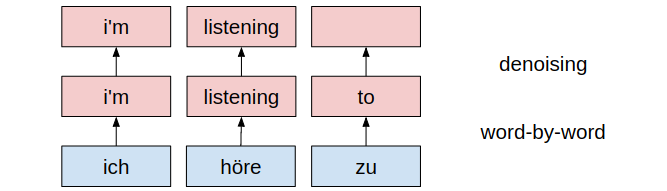
\includegraphics[width=0.8\linewidth]{insertion}
	\end{center}\vspace{0.5em}	
\end{itemize}

\vfill

%%%%%%%%%%%%%%%%%%%%%%%%%%%%%%%%%%%%%%%%%%%%%%%%%%%%%%%%%%%%%%%%%%%%%%%%%%%%%%%%%%%%%%%
\NewPage
\headline{Deletion}
\begin{itemize}
	\item Motivation
	\begin{itemize}
		\item In contrary case: some words are not related to any source word
	\end{itemize}
	
	\item Realization
	\begin{itemize}
		\item For each position in a sentence, delete the word according to a probability distribution ${p_{del}}$ as input
		\item  Denoising network learns to add some potential words when translating
	\end{itemize}	
	\begin{center}
		\vspace{0.5em}
		\hspace{-1cm}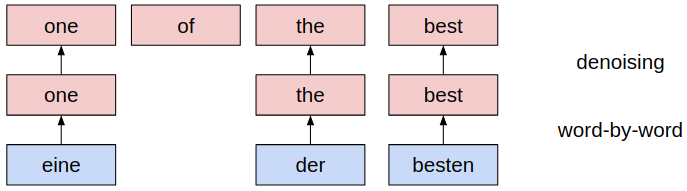
\includegraphics[width=0.8\linewidth]{deletion}
	\end{center}\vspace{0.5em}	
\end{itemize}

%%%%%%%%%%%%%%%%%%%%%%%%%%%%%%%%%%%%%%%%%%%%%%%%%%%%%%%%%%%%%%%%%%%%%%%%%%%%%%%%%%%%%%%
\NewPage
\headline{Reordering}	
\begin{itemize}
	\item Motivation
	\begin{itemize}
		\item Generated words are not in a correct sequence of the target language
	\end{itemize}
	\item Method
	\begin{itemize}
		\item For each position of a sentence, swap the words within a limited distance $d_{per}$ as input
		\item Denoising network learns reordering information when translating
	\end{itemize}
	\begin{center}
		\vspace{0.5em}
		\hspace{-1cm}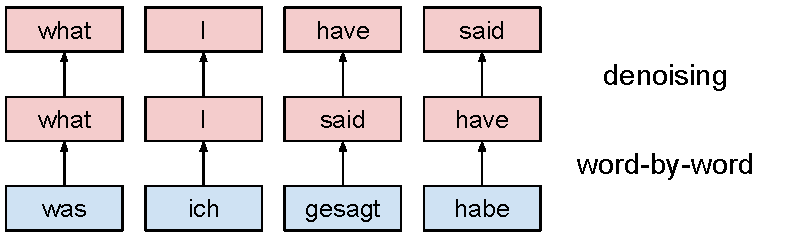
\includegraphics[width=0.8\linewidth]{denoising}
	\end{center}\vspace{0.5em}
\end{itemize}	

	%%%%%%%%%%%%%%%%%%%%%%%%%%%%%%%%%%%%%%%%%%%%
	\NewPage
	\headline{Corpus-based Leaning}	
	\vfill
	Motivation
	\begin{itemize}
		\item Vocabulary-based just looks at the mutual nearest neighbours
		\item Word frequency should also be accounted
		\item Assign priority to frequent words\\
	\end{itemize}
	Intuition
	\begin{itemize}
		\item Integrate the translation task into the learning process of cross-lingual word embedding
		\item Make use of Language Model
	\end{itemize}
	\vfill


	%%%%%%%%%%%%%%%%%%%%%%%%%%%%%%%%%%%%%%%%%%%%
	\NewPage
	\headline{Framework}	
	\vfill

		\centering
	\begin{minipage}{.7\linewidth}

			\begin{algorithm}[H]
				\SetAlgoLined
				\KwIn{$F$ (source embeddings)}
				\KwIn{$E$ (target embeddings)}
				\KwIn{$\textbf{LM}_e$ (language model)}
				\KwIn{$\mathcal{F}$ (source corpus)}
				\KwResult{$W$ (embedding mapping)}
				\While{not converge}{
					${\ \  \mathcal{E} \leftarrow TRANSLATE(\mathcal{F}, F, E, \textbf{LM}_e)}$ 
					${W \leftarrow LEARN\_MAPPING(\mathcal{F}, \mathcal{E})}$				
				}		
				\caption{Iterative learning of corpus-based approach}
			\end{algorithm}
	\end{minipage}
	\begin{itemize}
		\item Composes of mapping learning, dictionary induction and corpus translation
		\item Efficiency turns out to be critical because of the additional translation task 
	\end{itemize}

	\vfill
	
	%%%%%%%%%%%%%%%%%%%%%%%%%%%%%%%%%%%%%%%%%%%%
	\NewPage
	\headline{Online Training Algorithm}	
	\vfill

	\centering
	\begin{minipage}{.7\linewidth}
		\begin{algorithm}[H]
			\SetAlgoLined
			\KwIn{$F$ (source embeddings)}
			\KwIn{$E$ (target embeddings)}
			\KwIn{$\textbf{LM}_e$ (language model)}
			\KwIn{$\mathcal{F}$ (source corpus)}
			\KwResult{$W$ (embedding mapping) }
			\While{not converge}{
				\ \ Generate batch of source sentences $\{f_1^J\}$ from $\mathcal{F}$\\
				${\{e_1^I\} \leftarrow TRANSLATE(\{f_1^J\}, F, E, \textbf{LM}_e) }$ 
				${W \leftarrow LEARN\_MAPPING(\{f_1^J\}, \{e_1^I\})}$				
			}		
			\caption{Online learning for corpus-based approach}
		\end{algorithm}
	\end{minipage}
	
	\vfill	
	
	%%%%%%%%%%%%%%%%%%%%%%%%%%%%%%%%%%%%%%%%%%%%
	\NewPage
	\headline{Training Details}	
	\vfill
	\begin{itemize}
		\item Dictionary Induction: CSLS retrieval
		
		\item Corpus Translation: Simplified as word-by-word translation
		
		\item Optimization Objective 
		\item Orthogonal Constraint
		\[ W \leftarrow (1+\beta) W - \beta(WW^\top)W\] 
		\item Stop Criterion\\
		average cosine similarity
			
	\end{itemize}
	\vfill

	%%%%%%%%%%%%%%%%%%%%%%%%%%%%%%%%%%%%%%%%%%%%
	\NewPage
	\headline{Training Details}	
	\vfill
	\begin{itemize}
		\item Embedding Normalization\\
		Centering: mean word embedding should be no bias
		\item Dictionary Induction\\
		 CSLS retrieval
		\item Corpus Translation: Simplified as word-by-word translation\\
		We use the word-by-word translation framework implemented before, with this translation pair at each position is taken as word translation candidate 
		
		\item Optimization Objective \\
	\[ W = \argmin_{W \in \mathbb{R}^{d \times d}} \frac{1}{{\lvert \tilde{V} \rvert}} \sum_{n=1}^{\lvert \tilde{V} \rvert} l(W\bm{f}_n, \bm{e}_n) \]
		
	\end{itemize}
	\vfill	
	
	%%%%%%%%%%%%%%%%%%%%%%%%%%%%%%%%%%%%%%%%%%%%
	\NewPage
	\headline{Training Details}	
	\vfill
	\begin{itemize}
		\item Orthogonal Constraint
		\[ W \leftarrow (1+\beta) W - \beta(WW^\top)W\]
		where $\beta = 0.01$ is suggested, we find the orthogonal constraint make the training procedure converge successfully
		\item Learning Rate Scheduling 
		\begin{itemize}
			\item Starting with initial learning rate for each embedding training step
			\item Inherit learning rate from last training step
		\end{itemize}
		\item Stop Criterion\\
		Average cosine similarity between top 10k most frequent source words and corresponding translation
	\end{itemize}
	\vfill
	%%%%%%%%%%%%%%%%%%%%%%%%%%%%%%%%%%%%%%%%%%%%
	\NewPage
	\headline{Experiment Settings }	
	\vfill
	\begin{itemize}
	\item Word embedding and LM trained on \texttt{News Crawl 2014-2017} (100M)
	\item BLEU evaluated on German$\leftrightarrow$English \texttt{newstest2016}
	\item {Word accuracy evaluated on  dictionaries released by Facebook}
		\begin{itemize}
			\item Dictionary built with internal translation tool
			\item Each word has 1-4 word translation(s)
			\item Top-1 accuracy			
		\end{itemize}
	\item Context-aware beam search
	\begin{itemize}
		\item Lexicon candidates: 100
		\item Beam width: 10
	\end{itemize}

	 
	\end{itemize}
	\vfill
	%%%%%%%%%%%%%%%
	\NewPage
	\headline{Corpus Statistics}
	\vfill
\begin{table}[]
	\centering
	\scalebox{0.8}{
	\begin{tabular}{c|c|c|c|c}
		\hline
		\multirow{4}{*}{\textbf{Train}} & \textbf{}              & \textbf{German} & \textbf{English} & \textbf{French} \\ \cline{2-5} 
		& \textbf{Sentences}     & \textbf{100M}   & \textbf{100M}    & \textbf{100M}   \\ \cline{2-5} 
		& \textbf{Running Words} & \textbf{1880M}  & \textbf{2360M}   & \textbf{3017M}  \\ \cline{2-5} 
		& \textbf{Vocabulary}    & \textbf{1254k}  & \textbf{523k}    & \textbf{660k}   \\ \hline
	\end{tabular}
	}
\end{table}

\begin{table}[]
	\centering
	\scalebox{0.85}{
	\begin{tabular}{c|c|c|c|c|c}
		\hline
		\multirow{7}{*}{\textbf{Test}} & \textbf{}                      & \multicolumn{2}{c|}{\textbf{\texttt{newstest2016}}}    & \multicolumn{2}{c}{\textbf{\texttt{newstest2014}}}    \\ \cline{3-6} 
		& \multicolumn{1}{l|}{\textbf{}} & \textbf{German}       & \textbf{English}      & \textbf{French}       & \textbf{English}      \\ \cline{2-6} 
		& \textbf{Sentences}             & \textbf{2999}         & \textbf{2999}         & \textbf{3003}         & \textbf{3003}         \\ \cline{2-6} 
		& \textbf{Running Words}         & \textbf{62506}        & \textbf{64619}        & \textbf{81165}        & \textbf{71290}        \\ \cline{2-6} 
		& \textbf{Vocabulary Size}       & \textbf{11978}        & \textbf{8645}         & \textbf{10899}        & \textbf{9200}         \\ \cline{2-6} 
		& \textbf{OOV Rates}             & \textbf{4116 (6.6\%)} & \textbf{1643 (2.5\%)} & \textbf{1731 (2.1\%)} & \textbf{1299 (1.8\%)} \\ \cline{2-6} 
		& \textbf{LM perplexity}         & \textbf{211.0}        & \textbf{109.6}        & \textbf{51.2}         & \textbf{84.6}         \\ \hline
		\multicolumn{4}{l}{\textbf{Search vocabulary in testing: 50k (src/tgt)}} \\

	\end{tabular}
	}
\end{table}
	\vfill
%%%%%%%%%%%%%%%
\NewPage
\headline{Experiments: Translation}
\vfill

\begin{table}

	\caption{Translation results on German$\leftrightarrow$English \texttt{newstest2016} and French$\leftrightarrow$English \texttt{newstest2014}.}
	
	\scalebox{0.9}{
		\centering
	\begin{tabular}{>{\bfseries}l>{\bfseries}c>{\bfseries}c>{\bfseries}c>{\bfseries}c}
		\toprule
		 & de-en & en-de & fr-en & en-fr\\
		System   & \textsc{Bleu} [\%] & \textsc{Bleu} [\%] & \textsc{Bleu} [\%] & \textsc{Bleu} [\%]\\
		\midrule
		Word-by-Word   & 11.1 & 6.7 & 10.6 & 7.8\\
		\midrule
	+ LM (5-gram) + tgt w/ high LM score for OOV  & 12.9 & 8.9 & 12.7 & 10.0\\
	+ LM (5-gram) + copy from src for OOV		& 14.5 & 9.9 & 13.6 & 10.9\\
		\midrule
		\hspace{10pt}+ Denoising (RNN)  & 16.2 & 10.6 & 15.8 & 13.3 \\
		\hspace{10pt}+ Denoising (Transformer) & \leavevmode\color{blue}{17.2} & \leavevmode\color{blue}{11.0}& \leavevmode\color{blue}{16.5} & \leavevmode\color{blue}13.9 \\
		\midrule
		\cite{lample2017unsupervised} & 13.3 & 9.6 & 14.3 & 15.1\\
		\cite{artetxe2017unsupervised} & - & - & 15.6 & 15.1\\
		\bottomrule
	\end{tabular}
	}


	\label{tab:results}
\end{table}	
\vfill	

	%%%%%%%%%%%%%%%%%%%%%%%%%%%%%%%%%%%%%%%%%%%%
	\NewPage
	\headline{Experiments: Cross-lingual Word Embedding}	
	\vfill
	\begin{table}
		\caption{Cross-lingual Word Retrieval Accuracy}
		\centering
		\begin{tabular}{>{\bfseries}l>{\bfseries}l>{\bfseries}c>{\bfseries}c}
			\hline
			&                & De-En [\%]& En-De [\%]            \\ \hline
			\multirow{2}{*}{Corpus-based } & lr scheduler 1 & 60.37 & 60.67            \\ \cline{2-4} 
			& lr scheduler 2 & 51.50 & \textbackslash{} \\ \hline
			Corpus-based without LM              & lr scheduler 1 & 54.36 &        \textbackslash{}           \\ \hline
			Adversarial                            &                & 53.50 &       \textbackslash{}   \\ \hline
			Adversarial + Refinement               &                & 64.92 & \textbackslash{}    \\ \hline
			Supervised                             &                & 65.38 & \textbackslash{}  \\ \hline
		\end{tabular}
		
	\end{table}
	\vfill




	%%%%%%%%%%%%%%%%%%%%%%%%%%%%%%%%%%%%%%%%%%%%%%%%%%%%%%%%%%%%%%%%%%%%%%%%
	%%%%%%%%%%%%%%%%%%%%%%%%%%%%%%%%%%%%%%%%%%%%%%%%%%%%%%%%%%%%%%%%%%%%%%%%%%%%%%%%%%%%%%%
	\NewPage
	\headline {Conclusions}
	\vfill
	Comprehensive results
	\begin{itemize}
		\item Context-aware beam search with LM helps the lexicon choice
		\item Denoising networks aimed at insertion/deletion/reordering noise works for such problems in a small range of sentences\\
	\end{itemize}
	Ablation studies
	\begin{itemize}
		\item BPE embeddings performs worse than word embeddings, especially with smaller
		vocabulary size.
		\item Word-by-word translation with cross-lingual
embedding depends highly on the frequent word mappings
		\item Phrase embedding only helps in word-by-word translation with LM
	\end{itemize}
	\vfill


	
	

	%%%%%%%%%%%%%%%%%%%%%%%%%%%%%%%%%%%%%%%%%%%%%%%%%%%%%%%%%%%%%%%%%%%%%%%%%%%%%%%%
	\FinalPage
	

	
	
	%%%%%%%%%%%%%%%%%%%%%%%%%%%%%%%%%%%%%%%%%%%%%%%%%%%%%%%%%%%%%%%%%%%%%%%%%%%%%%%%
	\NewPage
	\bibliographystyle{i6bibliostyle}
	\bibliography{references}
	
\end{document}

%%%%%%%%%%%%%%%%%%%%%%%%%%%%%%%%%%%%%%%%%%%%%%%%%%%%%%%%%%%%%%%%%%%%%%%%%%%%%%%%%%%%%
%%%%%%%%%%%%%%%%%%%%%%%%%%%%%%%%%%%%%%%%%%%%%%%%%%%%%%%%%%%%%%%%%%%%%%%%%%%%%%%%
